%!TEX root = ../thesis.tex
\renewcommand{\Q}{\scr Q}

\section{The algorithm}

We will assume the entire graph has no seperating 3 or 4 cyles. We will show that in this case ...

\subsection{Definitions}
  \subsubsection{The neighbor walk of a path}
    \fxwarning{Note that the same/similar things hold for the left boundary walk}
    During this proof we will frequently use the concept of the left or right neighbor walk of a path.
    Given a path $P = p_1 \ldots p_k$ in a graph $G$
    The \emph{right neighbor walk} $W$ of $P$ will consist of $p_1$ and the vertices adjacent to $p_{2}$ between $p_1$ and $p_{3}$ in the clockwise rotation at $p_{2}$ followed by the vertices between $p_{2}$ and $p_{4}$ in the rotation at $p_{3}$ and so further until we add the vertices between $p_{k-2}$ and $p_k$ in the rotation around $p_{k-1}$ and finally we finish by adding $p_k$ to $W$.
    We then remove all subsequent duplicates from $W$

    \begin{lemma}
      \label{lm:uni:neighborWalk}
      The right neighbor walk $W$ is a walk.
    \end{lemma}
    \begin{proof}
      Let $w$ and $w'$ be two subsequent vertices in $W$. We will show they are connected. We first consider the case $\braces{w, w'} \cap \braces{p_1, p_k } = \emptyset$.
      Now there are two cases. Either $(a)$ $w$ and $w'$ are vertices adjacent to some $p_i$ an thus subsequent in the rotation at $p_i$  or $(b)$ $w$ was the last vertex adjacent to some $p_i$ and thus $w'$ is the first vertex adjacent to $p_{i+1}$.

      The following two situations can also be seen in Figure \ref{fig:uni:walkproof}.

      \begin{figure}[h]
          \centering
          \begin{subfigure}[b]{0.5\linewidth}
              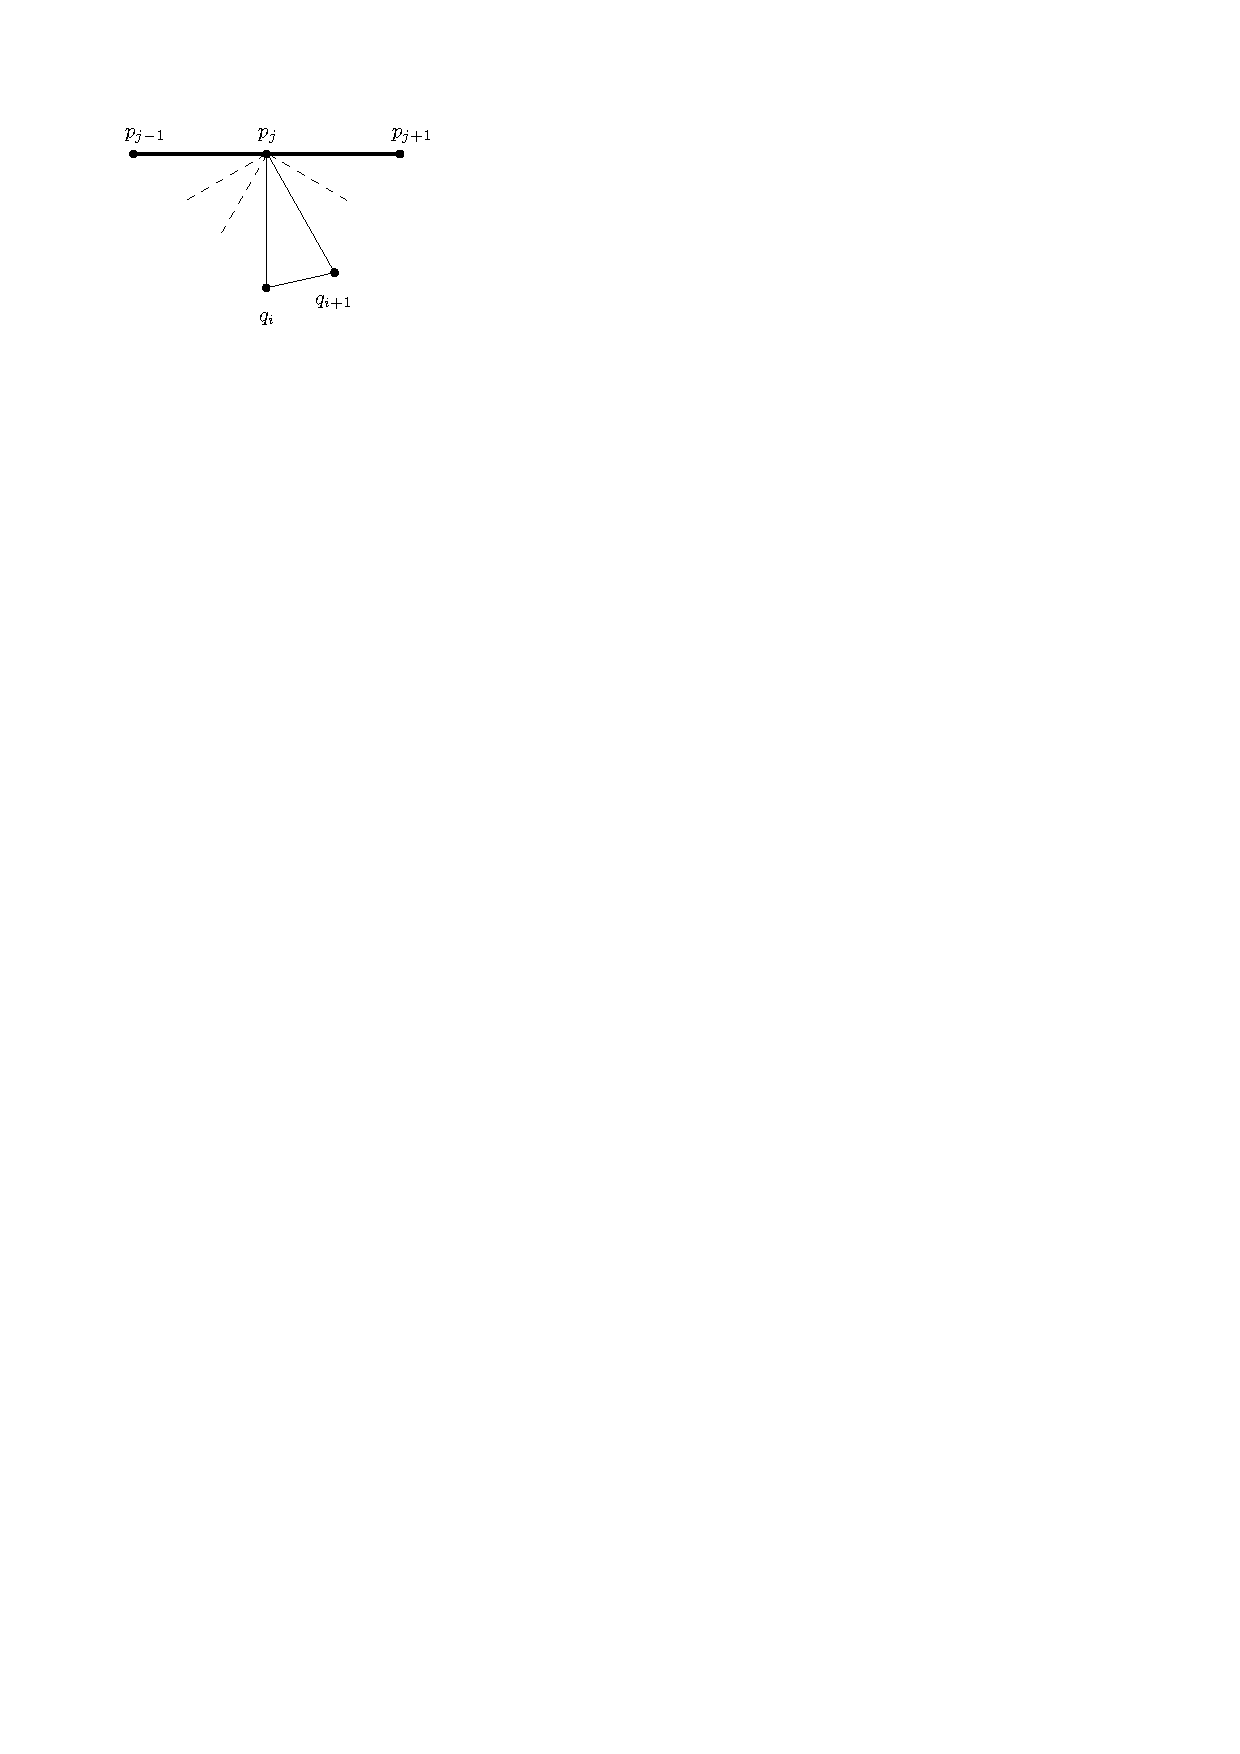
\includegraphics[width=\linewidth]{unifiedAlgo/img/walkProofA}
              \caption{}
          \end{subfigure}%
          \begin{subfigure}[b]{0.5\linewidth}
              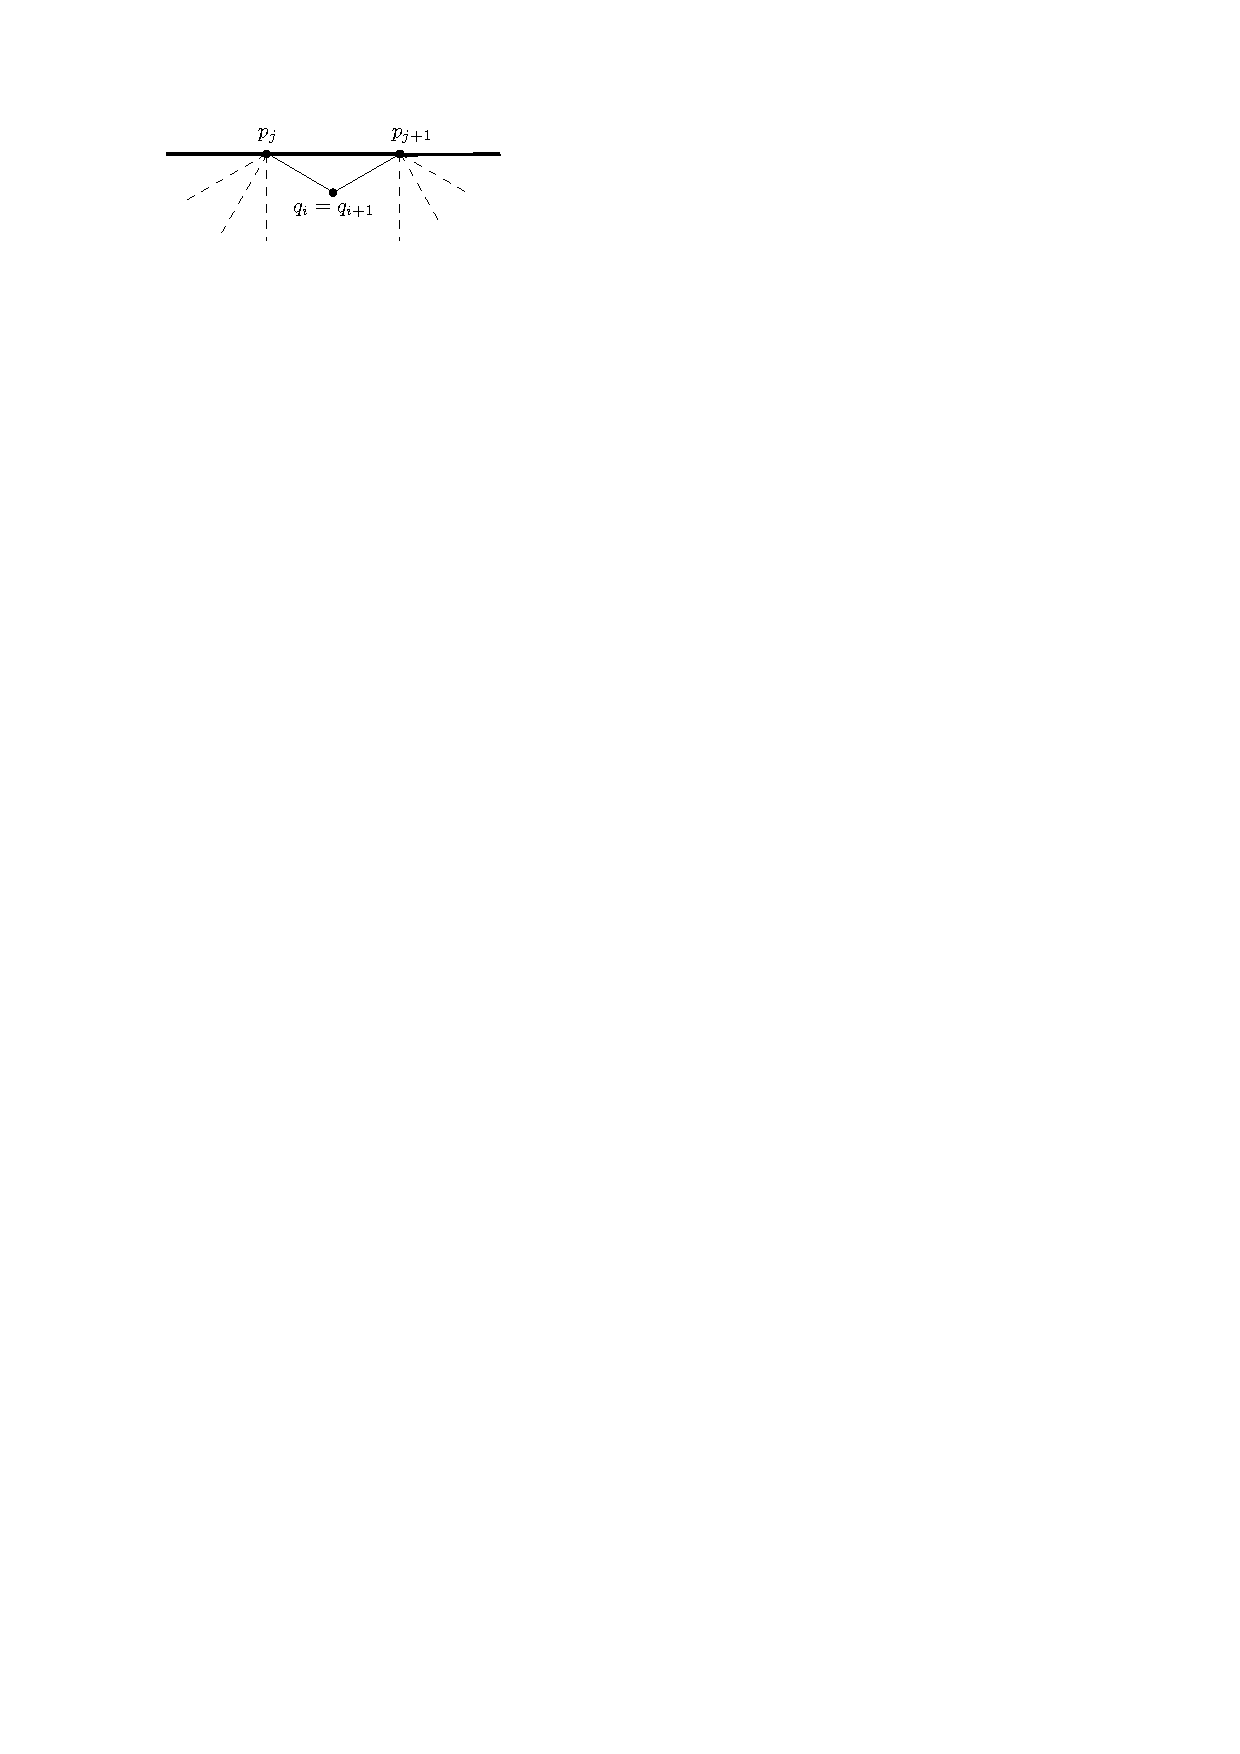
\includegraphics[width=\linewidth]{unifiedAlgo/img/walkProofB}
              \vspace{1cm}

              \caption{}
          \end{subfigure}

            \caption{The two main cases of the proof showing that $W$ is a walk}
        \label{fig:uni:walkproof}
      \end{figure}

      In case $(a)$ we note that since $w$ and $w'$ are subsequent in the rotation at $p_i$ $ww'$ is an edge by Lemma \ref{lm:prelim:rotationEdge}.

      In case $(b)$ we note that $p_i w$ and $p_i p_{i+1}$ are edges subsequent in clockwise order, hence $wp_{i+1}$ is also an edge. Hence $w$ is the first vertex adjacent to $p_{i+1}$ subsequent to $v_i$ in the clockwise rotation. Thus $w= w'$. They are duplicates and one of them must have been removed.

      Now for the edge cases: Let $x$ be the first vertex adjacent to $p_{i+1}$ and let $y$ be the last vertex adjacent to $p_{j-1}$. $p_i$ and $x$ are vertices adjacent to $p_{i+1}$ subsequent in the clockwise rotation, and hence connected by Lemma \ref{lm:prelim:rotationEdge}. In the same way $y$ and $v_j$ are subsequent vertices in the rotation at $v_n$ and hence connected.

      Hence $\W$ is a walk.
    \end{proof}


    \begin{lemma}
      \label{lm:uni:neighborWalkNoncrossing}
      The right neighbor walk $W$ is a non-crosssing walk.
    \end{lemma}
    \begin{proof}
      Suppose that the right neighbor walk is crossing at a vertex $w= w_i =w_j$. Then one of $w_{j-1}$ and $w_{j+1}$ is in the clockwise interval $[w_{i-1}, w_{i+1} ]$ at the rotation at $w$. We will denote this vertex by $w'$. It is clear that $w'$ cannot be on the path unless $w'$ is $p_1$ or $p_k$. In this case however we see that $w_{i-1}$ or $w_{i+1}$ respectively couldn't have been part of the path.

      So we continue with $w'$ not on the path. All neighbors of $w$ between $w_{i-1}$ and $w_{i+1}$ in the clockwise rotation are on the path. \fxwarning{TODO make this a lemma}. So we have a series of triangles by Lemma \ref{lm:prelim:rotationEdge}. Now $w'$ must be inside one of these triangles, otherwise we would have a crossing edge (and thus a non-planar graph.) Now the triangle containing $w$ is a separating triangle.

      We conclude that $W$ must be a non-crossing walk.
    \end{proof}


    \fxnote{Actullly W rev(P)}
    \begin{lemma}
      \label{lm:uni:neighbourwalkNoInteriorVertex}
      The closed non-crosing walk $WP$ has no interior vertex.
    \end{lemma}
    \begin{proof}subsequent
      The interior of $WP$ consists of only triangles with all vertices in $WP$. We can see this from the construction of the neighbor walk. Both cases in Figure \ref{fig:uni:walkproof} add a triangle to the interior with all vertices in $WP$.

      Suppose there is a interior vertex. Then the triangle containing this vertex is a separating triangle.
    \end{proof}


    \begin{lemma}
      \label{lm:uni:neighbourwalkChordFree}
      The left of the of a right neighbor walk and the right of the left neighbor walk are chordfree.
    \end{lemma}
    \begin{proof}
      Suppose that the right neighbor walk $W = w_1 \ldots w_k$  has a chord on the left, say between $w_i$ and $w_j$ with $i< j -1 $. There is a vertex $p_\ell \in P$ on the path such that $w_{i+1}$ is a neighbor of $p_\ell$ to the left of $p_\ell$ Consider now the following non-crossing closed walk $P w_k \ldots w_{j+1} w_j w_i w_{i-1} \ldots w_1$
      (Thick in Figure \ref{fig:uni:neihbourwalkChordFree})this walk has $w_{i+1}$ in its exterior. But then $p_\ell w_{i+1}$ is a crossing edge. Which is forbidden.

      \begin{figure}[h]
        \centering
        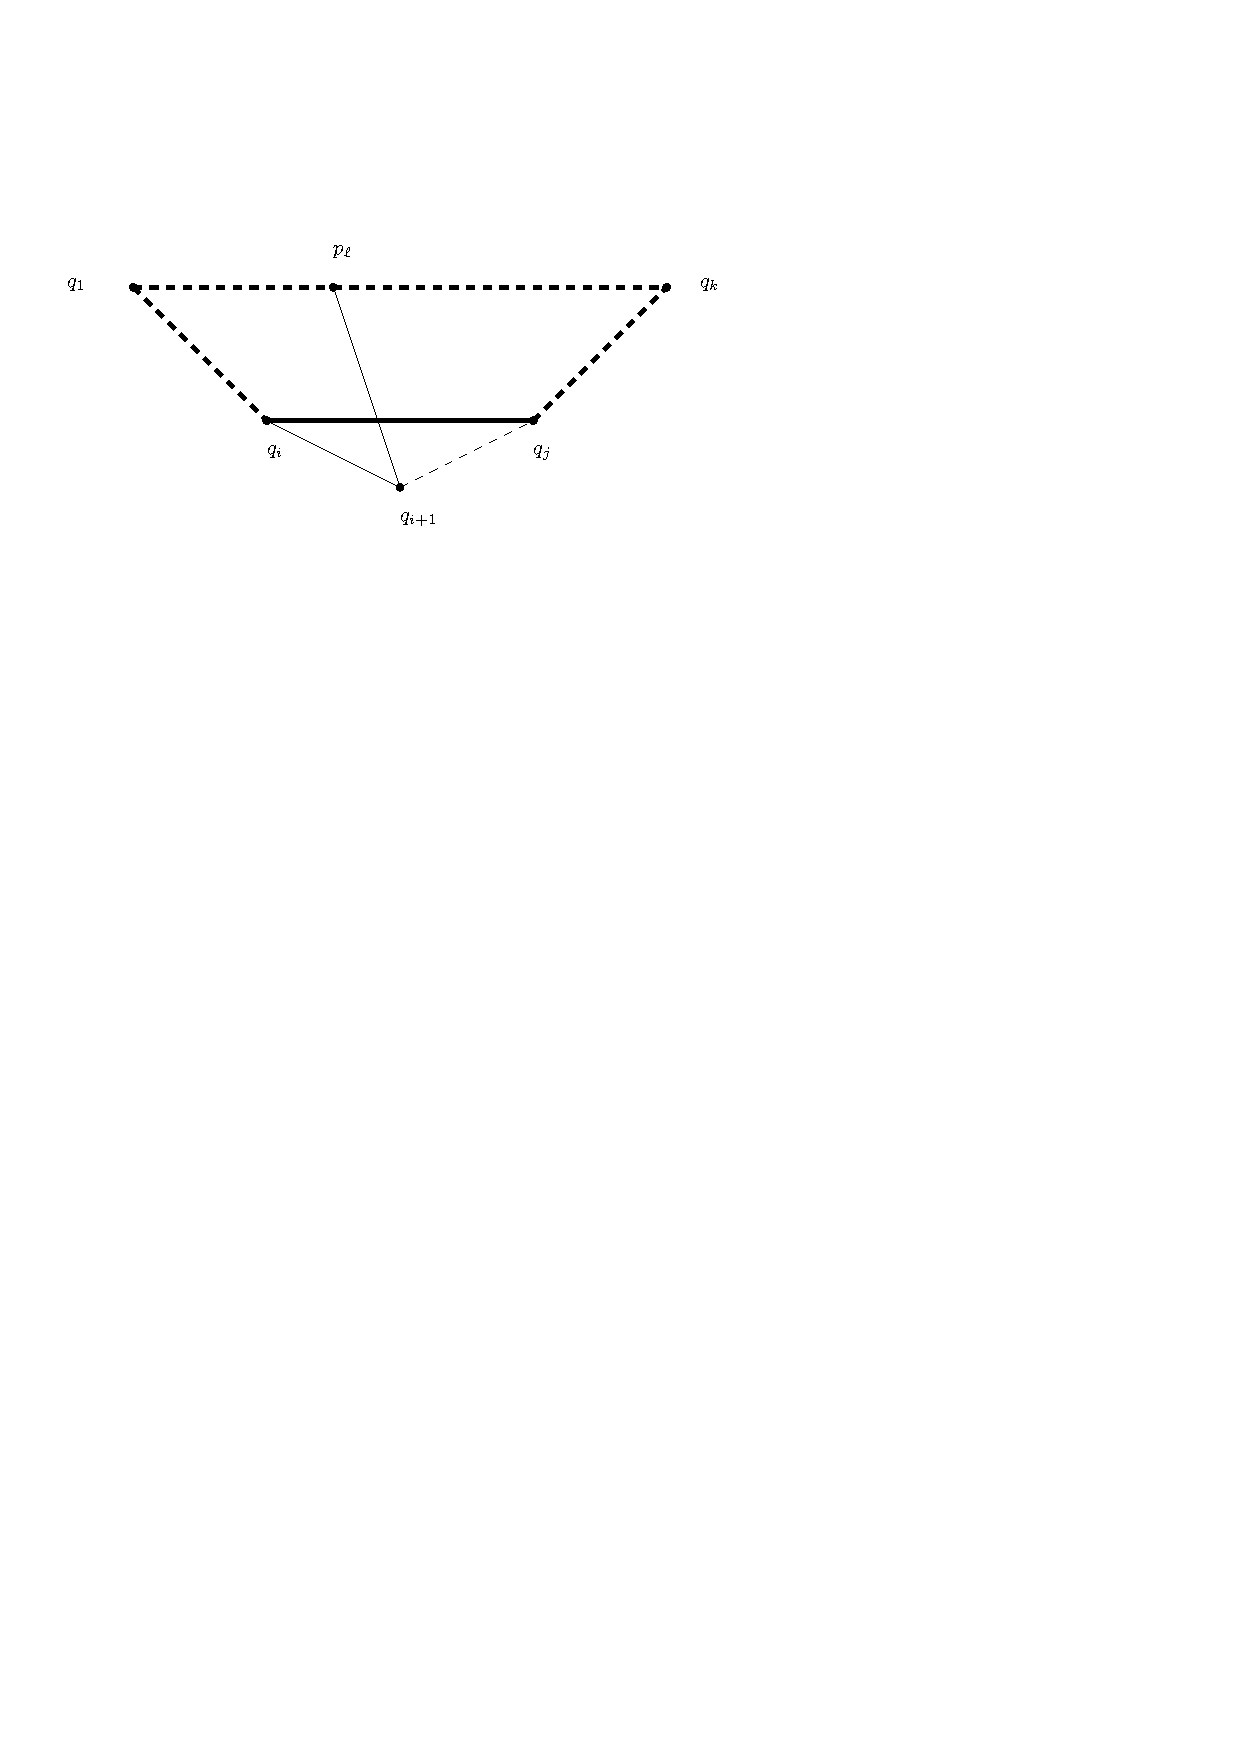
\includegraphics[scale=1]{unifiedAlgo/img/neighbourWalkChords}
        \caption{The construction in the proof of Lemma \ref{lm:uni:neighbourwalkChordFree}}
        \label{fig:uni:neihbourwalkChordFree}
      \end{figure}
    \end{proof}

    \fxnote{Alternate proof based on   ($\W$ being oriented from $\pW$ to $\pE$), since if it would lie on the left of $\W$ the vertices $w_{i+1},\ldots, w_{j-1}$ would not have been chosen in the construction of the prefence.}

  \subsubsection{More chords}
    Recall that a \emph{chord} of a path $\P$ is a edge that connects two non-subsequent vertices of that path. Note that this edge can't be in the path. A \emph{k-chord} is a path $\Q$ of $k$ edges that connects two nonsubsequent vertices $v_i, v_j$ of the path such that $\P \cap \Q = \braces{v_i, v_j}$.

    Note that $\P|_{v_i, v_j} \oplus \rev(\Q)$ is a cycle. We call this chord \emph{separating} if this is a separating cycle. \fxnote{Define Rev}

  %  We call a chord \emph{unaivoidable} if on the other side of the path $v_i$ and $v_j$ are connected with an $2-chord$. That is, a $3$-chord on the right of $\P$ is unavoidable if there is a $2-chord$ on the left of $\P$. \fxnote{Figure of this situation, two non-seperating chords}

\subsection{Outline}
  The algorithm will consist of two phases

  \begin{enumerate}
    \item Find a \emph{vertically} 1-sided layout with additional properties
    \item Do additional post-processing steps to make this layout $k$-sided.
  \end{enumerate}

\subsection{Description Phase 1}
  In Phase 1 we execute a sweepcycle algorithm comparable to Fusy's \cite{Fusy2006}.
  During the algorithm we will want to maintain several invariants. The first three are equivalent to those imposed by Fusy. The final two invariants are new and impose a nice structure on the sweepcycle so far.

  \begin{invariants}
    \itemsep=-4pt

    \item \label{i:uni:SWandSE} The cycle $\C$ contains the two edges $\pS \pW$ and $\pS \pE$.
    \item \label{i:uni:noChords} $\cpath$ has no chords
    \item \label{i:uni:intVertCond} All inner edges of $T$ outside of $\C$ are colored and oriented in such that the inner vertex condition holds. %TODO what is the inner vertex condition
    \fxerror{We need to add a partial inner vertex condition}
    \item \label{i:uni:no2Chords} $\C\sm{\pW, \pS, \pE}$ has no separating 2-chords
    %\item \label{i:uni:no3chords} $\cpath$ has no avoidable separating 3-chords
  \end{invariants}





  \begin{defi}[Prefence]
  A prefence $\W$ is a interior path of $\C$ starting at $v_i \in \C$ and ending at $v_j \in \C$ a both adjacent to $\pS$
  \begin{enumerate}
   \renewcommand*{\labelenumi}{(P\arabic{enumi})}%
   \renewcommand*{\theenumi}{(P\arabic{enumi})}%
    \item  $\C_\W$ Has no interior vertex
    \label{p:noInteriorVertex}
    \item  $\W$ has no chords on the left     \label{p:Wchordfree}

    \item  $\restC{\W}$ has no chords on the right     \label{p:Cchordfree}

  \end{enumerate}
  \end{defi}

  We do the following
  \begin{enumerate}
    \item Find the right neighbor walk
    \item Evade any future irregularities
    \item Update with this valid path
  \end{enumerate}

  We then repeat this until the sweepcycle does not contain any more interior vertices.

  \paragraph{Find the right neighbor path}
    Let $v_i$ denote all the vertices of $\cpath$ in the following order $\pW =  v_1 \  v_2 \  \ldots v_{n-1} \  v_n = \pE$.
    Some intervals of these vertices will be adjacent to $\pS$. However, they can't be all adjacent to $S$ since then the sweepcycle would be non-separating since we can't have separating triangles. We denote by $v_i$ the last vertex of fist interval of vertices adjacent to $S$ and by $v_j$ the first vertex of the second interval.
    As candidate walk we will take the right neighbor path of $C\sm{S, v_1, \ldots v_{i-1}, v_{j+1}, \dots v_n}$.
    \fxnote{beter notation}

    \begin{lemma}
      \label{lm:uni:isPrefence}
    The collection $W$ described above is a prefence.
    \end{lemma}
    \begin{proof}
    $W$ is a walk by lemma \ref{lm:uni:neighborWalk}. Furthermore it is a path since any non-simple point would offend Invariant \ref{i:uni:no2Chords} of the sweepcycle.


    We note \ref{p:noInteriorVertex} holds due to Lemma \ref{lm:uni:neighbourwalkNoInteriorVertex}

    We note \ref{p:Wchordfree} holds due to Lemma \ref{lm:uni:neighbourwalkChordFree}.

    We note \ref{p:Cchordfree} holds due to invariant \ref{i:uni:noChords}.
    \end{proof}

    We then orient $\W$ from $v_i$ (the vertex closest to $\pW$)to $v_j$ (the vertex closest to $\pE$) and denote it's vertices by $w_1 \ldots w_k$.


    \subsubsection{Irregularities}
      Now the prefence we found can have several structures we want to avoid
      namely
      \begin{enumerate}
        \itemsep=-4pt
        \item Chords
        \item Separating 2-chords
      \end{enumerate}

      All of these structures are on the right of the prefence since the prefence satisfies \ref{p:Wchordfree} (no chords on the left) and \ref{p:noInteriorVertex} (no separating 2-chords on the left).

      What we do depends on the first obstacle we encounter. The range of an obstcle will be given by it's start  and end vertex.

      \paragraph{First obstacle is a chord}
      If our precycle has any chords we look identify the them by their start and end vertex. Of the chords with the lowest start index we will consider the one with the largest end index.

      Now we have a group of chords with start and end vertices. What we do now depends on whether a 2-chord shows up.

      \emph{No 2-chord}
      We look at the chord with the smallest range (i.e. highest start $i_0$ and lowest end $j_0$) then we will look at the biggest chords still starting at $i_0$ or ending at $j_0$. Say that this chord goes from $i_1$ to $j_1$ then we augment the sweepcycle with $i_1 +1$ to $j_1 -1$.

      \emph{A 2-chord}
      We find a piece to augment with in the same way  but we terminate it just before the first closing 2-chord.

      \paragraph{First obstacle is a 2-chord}
      If this 2-chord contains a chord, just apply the rules for chords as given above. Otherwise terminate the prefence just before the end of the 2-chord.


    \begin{lemma}
      \label{lm:}
      We always augment with a valid path
    \end{lemma}
    \begin{proof}
      By construction
    \end{proof}

    \begin{lemma}
      \label{lm:}
      The resulting REL is vertically one-sided
    \end{lemma}
    \begin{proof}
      This is the same as saying that the resulting regular edge labeling has no blue Z's

      There are two ways a blue Z can form either we start at a vertex just before a merge or we terminate on a vertex just after a split.

      For start point the following holds. Either we start adjacent to $\pS$ or we start due to a chord.

      For end points the following holds either we end adjacent to $\pS$, or due to a chord or 2-chord.


      We will first show that we can't have a start just after a merge.
      If the merge is due to the vertex being adjacent to $\pS$ then the previous vertex is also adjacent to $\pS$ and we have nowhere to go. \fxnote{provide figure}

      Suppose now we ended due to a chord or a 2-chord. Then the only reason to start on this place is due to a chord.

      If we start or end at a vertex adjacent to $\pS$ the diagonal edge can't exist. Because there is not enough space for moves that could have generated this ... (I Think)

      \fxerror{Work this out, no energy now}


    \end{proof}


\subsection{Proofs Phase 1}

\subsection{Phase 2}
We will then show the following

\begin{lemma}
  \label{lm:}
  Given a vertically one-sided REL we can produce a REL that is vertically 2-sided and in which all horizontal faces that are not 2-sides don't contain botomfans larger than 5.
\end{lemma}
\begin{proof}
  There is an ordering on the strips in the REL, namely the order in which they are created. Such that every strip is larger then those above it and smaller then those below it.

  We will start our procedure in the largest strip and go down the order.

  For every strip we do the following:
  \begin{enumerate}
    \item Flip the edges next to each large bottomfan. Unless this crates a mono-colored triangle.
    \item Check for $Z$'s  in the same direction in this strip and a higher strip and remove them.
    \item Check for subsequent $Z$'s in the opposite direction.
    \item Check for a $Z$ with a large left-fan
  \end{enumerate}

  For the way we flip around bottomdfans one can also consult Figure \ref{fig:uni:bottomFanFlips}.

  After these flips we can have a number of undiserable structures. Please refer to Figure \ref{fig:uni:undesirableStructures}.

  \begin{figure}[h]
    \centering
    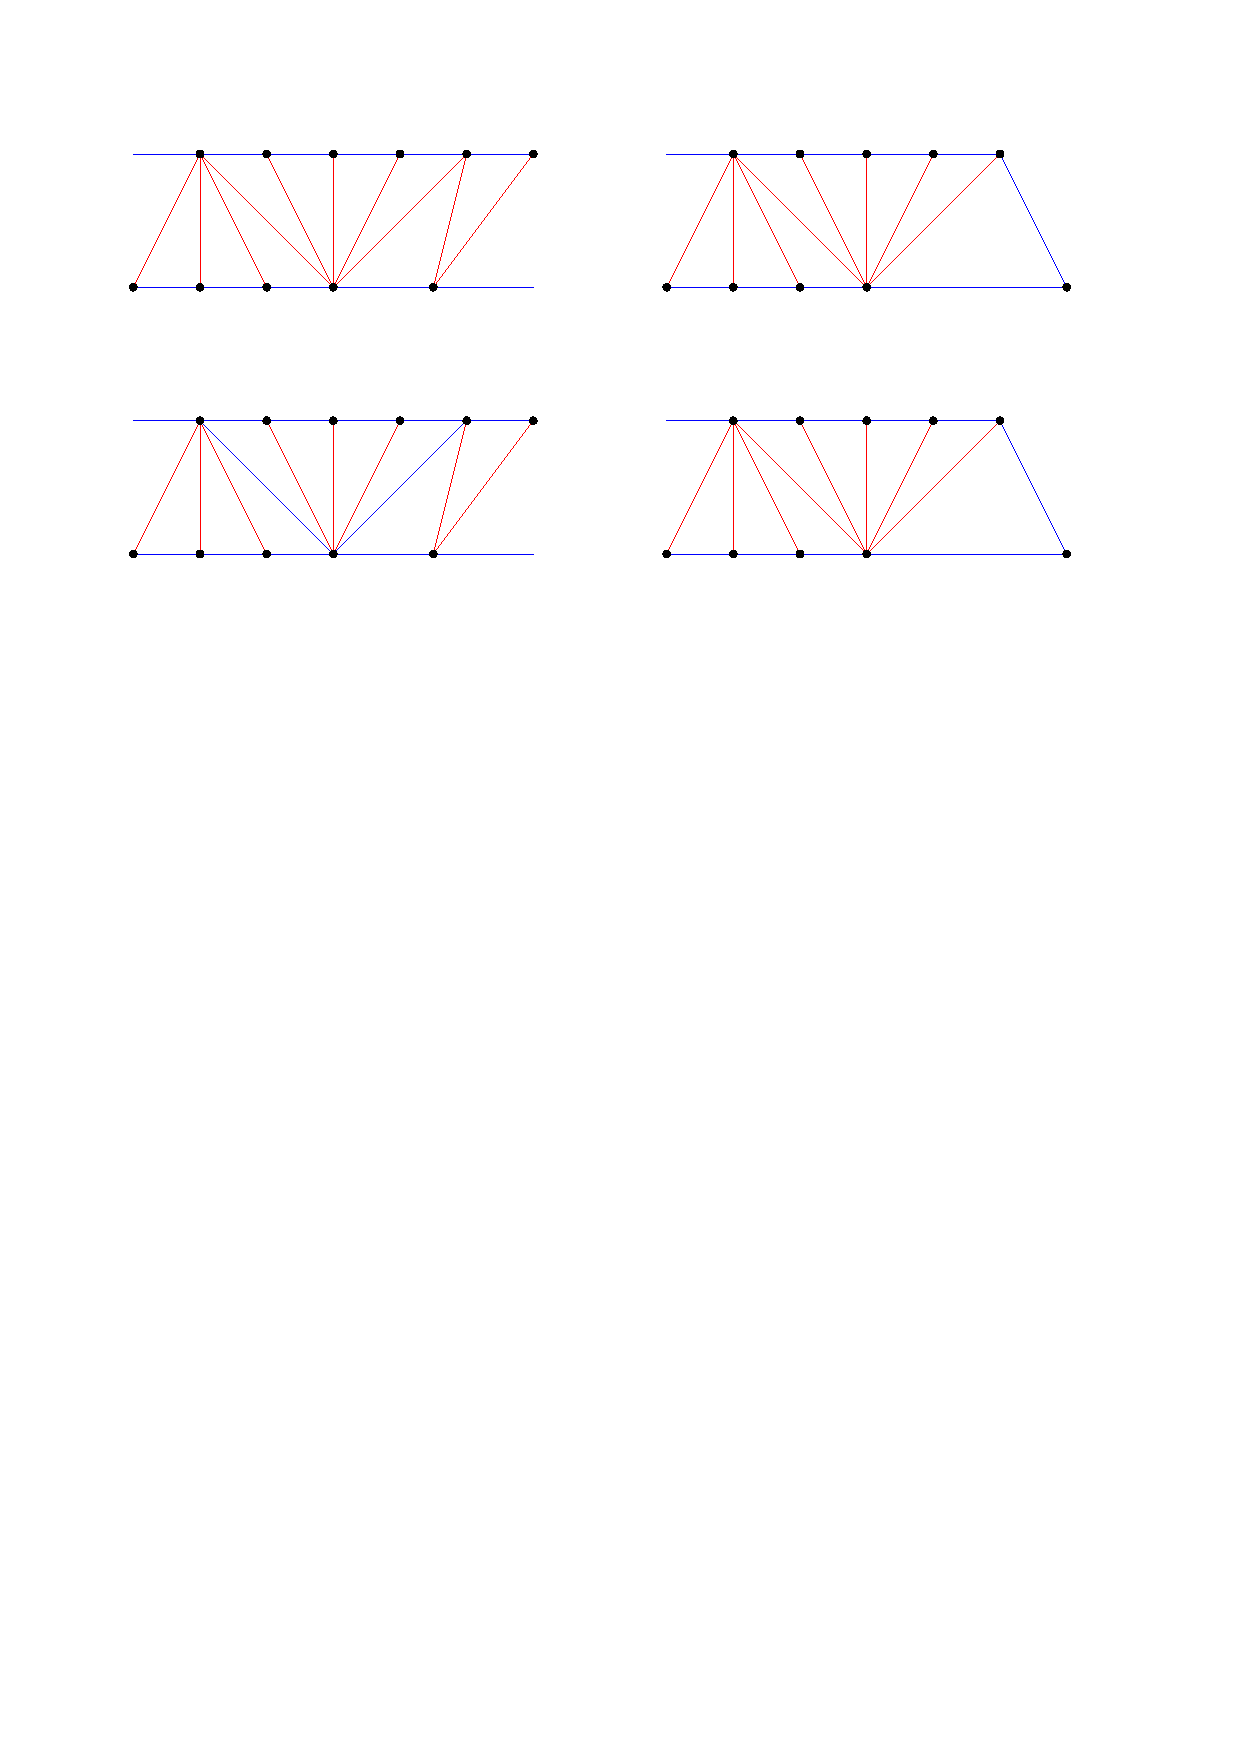
\includegraphics[scale=1]{unifiedAlgo/img/bottomFanFlips}
    \caption{Flipping around bottom-fans}
    \label{fig:uni:bottomFanFlips}
  \end{figure}

  \begin{figure}
      \centering
      \begin{subfigure}[b]{0.45textwidth}
          \includegraphics[width=textwidth]{}
          \caption{}
      \end{subfigure}
      ~
      \begin{subfigure}[b]{0.45textwidth}
          \includegraphics[width=textwidth]{}
          \caption{}
      \end{subfigure}
      	\caption{}
  \label{fig:uni:undesirableStructures}
  \end{figure}
\end{proof}
